\documentclass{standalone}
\usepackage{tikz}
\usetikzlibrary{patterns, positioning}
\usepackage[sfdefault]{ClearSans} %% option 'sfdefault' activates Clear Sans as the default text font
\usepackage[T1]{fontenc}

\begin{document}
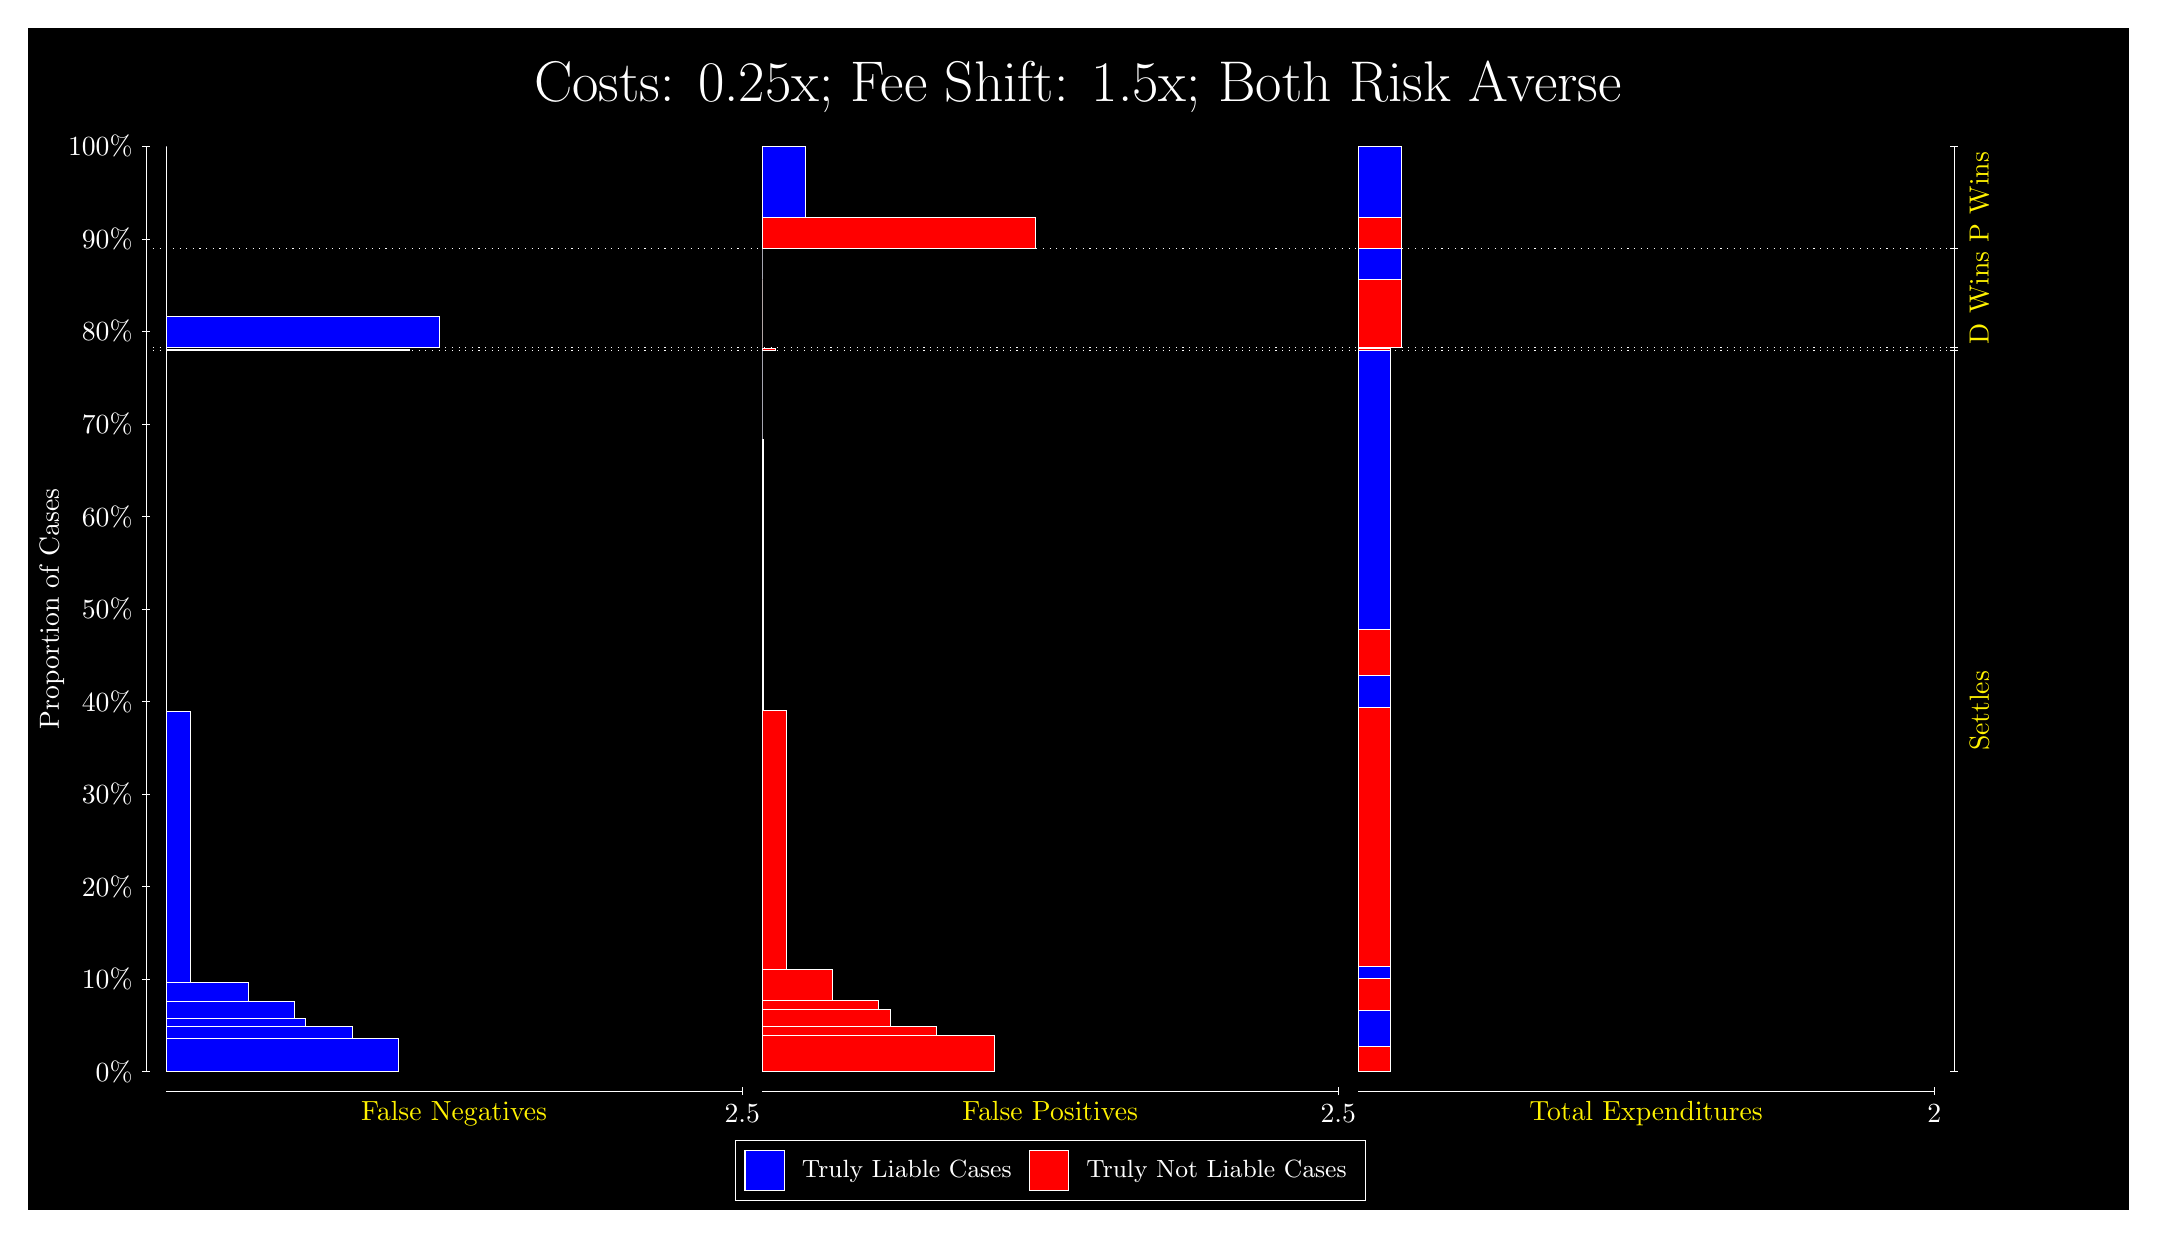
\begin{tikzpicture}
\draw[fill=black] (0,0) rectangle (26.667,15);
\draw[text=white] (0,13.5) rectangle (26.667,15) node[midway] {\huge Costs: 0.25x; Fee Shift: 1.5x; Both Risk Averse};
\draw[white, very thin] (1.5,1.75) -- (1.5,13.5);
\node[rotate=90, text=white, anchor=center] at (0.3, 7.625) {Proportion of Cases};
\draw[white, very thin] (1.45,1.75) -- (1.55,1.75);
\node[text=white, anchor=east] at (1.45, 1.75) {0\%};
\draw[white, very thin] (1.45,2.925) -- (1.55,2.925);
\node[text=white, anchor=east] at (1.45, 2.925) {10\%};
\draw[white, very thin] (1.45,4.1) -- (1.55,4.1);
\node[text=white, anchor=east] at (1.45, 4.1) {20\%};
\draw[white, very thin] (1.45,5.275) -- (1.55,5.275);
\node[text=white, anchor=east] at (1.45, 5.275) {30\%};
\draw[white, very thin] (1.45,6.45) -- (1.55,6.45);
\node[text=white, anchor=east] at (1.45, 6.45) {40\%};
\draw[white, very thin] (1.45,7.625) -- (1.55,7.625);
\node[text=white, anchor=east] at (1.45, 7.625) {50\%};
\draw[white, very thin] (1.45,8.8) -- (1.55,8.8);
\node[text=white, anchor=east] at (1.45, 8.8) {60\%};
\draw[white, very thin] (1.45,9.975) -- (1.55,9.975);
\node[text=white, anchor=east] at (1.45, 9.975) {70\%};
\draw[white, very thin] (1.45,11.15) -- (1.55,11.15);
\node[text=white, anchor=east] at (1.45, 11.15) {80\%};
\draw[white, very thin] (1.45,12.325) -- (1.55,12.325);
\node[text=white, anchor=east] at (1.45, 12.325) {90\%};
\draw[white, very thin] (1.45,13.5) -- (1.55,13.5);
\node[text=white, anchor=east] at (1.45, 13.5) {100\%};

\draw[white, very thin] (24.457,1.75) -- (24.457,13.5);
\draw[white, very thin] (24.407,1.75) -- (24.507,1.75);
\node[anchor=west] at (24.407, 1.75) {};
\draw[white, very thin] (24.407,10.911) -- (24.507,10.911);
\node[anchor=west] at (24.407, 10.911) {};
\draw[white, very thin] (24.407,10.943) -- (24.507,10.943);
\node[anchor=west] at (24.407, 10.943) {};
\draw[white, very thin] (24.407,12.207) -- (24.507,12.207);
\node[anchor=west] at (24.407, 12.207) {};
\draw[white, very thin] (24.407,13.5) -- (24.507,13.5);
\node[anchor=west] at (24.407, 13.5) {};

\draw[white, very thin, fill=blue] (1.75,1.75) rectangle (4.6958,2.1663);
\draw[white, very thin, fill=blue] (1.75,2.1663) rectangle (4.1103,2.3194);
\draw[white, very thin, fill=blue] (1.75,2.3194) rectangle (3.5248,2.4214);
\draw[white, very thin, fill=blue] (1.75,2.4214) rectangle (3.3784,2.6403);
\draw[white, very thin, fill=blue] (1.75,2.6403) rectangle (2.7929,2.8793);
\draw[white, very thin, fill=blue] (1.75,2.8793) rectangle (2.0611,6.3241);
\draw[white, very thin, fill=red] (1.75,6.3241) rectangle (1.75,10.911);
\draw[white, very thin, fill=blue] (1.75,10.911) rectangle (4.8422,10.919);
\draw[white, very thin, fill=red] (1.75,10.919) rectangle (1.75,10.943);
\draw[white, very thin, fill=blue] (1.75,10.943) rectangle (5.2265,11.341);
\draw[white, very thin, fill=red] (1.75,11.341) rectangle (1.75,12.207);
\draw[white, very thin, fill=red] (1.75,12.207) rectangle (1.75,12.605);
\draw[white, very thin, fill=blue] (1.75,12.605) rectangle (1.75,13.5);
\draw[white, very thin, fill=red] (9.3189,1.75) rectangle (12.265,2.2125);
\draw[white, very thin, fill=red] (9.3189,2.2125) rectangle (11.533,2.3194);
\draw[white, very thin, fill=red] (9.3189,2.3194) rectangle (10.947,2.5383);
\draw[white, very thin, fill=red] (9.3189,2.5383) rectangle (10.801,2.6532);
\draw[white, very thin, fill=red] (9.3189,2.6532) rectangle (10.215,3.0528);
\draw[white, very thin, fill=red] (9.3189,3.0528) rectangle (9.6299,6.3372);
\draw[white, very thin, fill=blue] (9.3189,6.3372) rectangle (9.3372,9.782);
\draw[white, very thin, fill=blue] (9.3189,9.782) rectangle (9.3189,10.911);
\draw[white, very thin, fill=red] (9.3189,10.911) rectangle (9.4835,10.935);
\draw[white, very thin, fill=blue] (9.3189,10.935) rectangle (9.3189,10.943);
\draw[white, very thin, fill=red] (9.3189,10.943) rectangle (9.3189,11.81);
\draw[white, very thin, fill=blue] (9.3189,11.81) rectangle (9.3189,12.207);
\draw[white, very thin, fill=red] (9.3189,12.207) rectangle (12.795,12.605);
\draw[white, very thin, fill=blue] (9.3189,12.605) rectangle (9.8678,13.5);
\draw[white, very thin, fill=red] (16.888,1.75) rectangle (17.299,2.0758);
\draw[white, very thin, fill=blue] (16.888,2.0758) rectangle (17.299,2.5338);
\draw[white, very thin, fill=red] (16.888,2.5338) rectangle (17.299,2.9334);
\draw[white, very thin, fill=blue] (16.888,2.9334) rectangle (17.299,3.0865);
\draw[white, very thin, fill=red] (16.888,3.0865) rectangle (17.299,6.371);
\draw[white, very thin, fill=blue] (16.888,6.371) rectangle (17.299,6.7872);
\draw[white, very thin, fill=red] (16.888,6.7872) rectangle (17.299,7.3646);
\draw[white, very thin, fill=blue] (16.888,7.3646) rectangle (17.299,10.911);
\draw[white, very thin, fill=red] (16.888,10.911) rectangle (17.299,10.935);
\draw[white, very thin, fill=blue] (16.888,10.935) rectangle (17.299,10.943);
\draw[white, very thin, fill=red] (16.888,10.943) rectangle (17.437,11.81);
\draw[white, very thin, fill=blue] (16.888,11.81) rectangle (17.437,12.207);
\draw[white, very thin, fill=red] (16.888,12.207) rectangle (17.437,12.605);
\draw[white, very thin, fill=blue] (16.888,12.605) rectangle (17.437,13.5);
\draw[white, dotted] (1.5,10.911) -- (24.457,10.911);
\draw[white, dotted] (1.5,10.943) -- (24.457,10.943);
\draw[white, dotted] (1.5,12.207) -- (24.457,12.207);
\draw[white, very thin] (1.75,1.5) -- (9.0689,1.5);
\node[text=yellow, anchor=north] at (5.4094, 1.5) {False Negatives};
\draw[white, very thin] (9.0689,1.45) -- (9.0689,1.55);
\node[text=white, anchor=north] at (9.0689, 1.45) {2.5};

\draw[white, very thin] (9.3189,1.5) -- (16.638,1.5);
\node[text=yellow, anchor=north] at (12.978, 1.5) {False Positives};
\draw[white, very thin] (16.638,1.45) -- (16.638,1.55);
\node[text=white, anchor=north] at (16.638, 1.45) {2.5};

\draw[white, very thin] (16.888,1.5) -- (24.207,1.5);
\node[text=yellow, anchor=north] at (20.547, 1.5) {Total Expenditures};
\draw[white, very thin] (24.207,1.45) -- (24.207,1.55);
\node[text=white, anchor=north] at (24.207, 1.45) {2};

\node[text=yellow, centered, rotate=90] at (24.777, 6.3307) {Settles};

\node[text=yellow, centered, rotate=90] at (24.777, 11.575) {D Wins};
\node[text=yellow, centered, rotate=90] at (24.777, 12.854) {P Wins};

\draw (12.978300999999998,1.5) node[draw=none] (baseCoordinate) {};
\begin{scope}[align=center]
        \matrix[scale=0.5, draw=white, below=0.5cm of baseCoordinate, nodes={draw}, column sep=0.1cm]{
            \node[rectangle, draw, minimum width=0.5cm, minimum height=0.5cm, fill=blue] {}; &
            \node[draw=none, font=\small, text=white] (B) {Truly Liable Cases}; &
            \node[rectangle, draw, minimum width=0.5cm, minimum height=0.5cm, fill=red] {}; &
            \node[draw=none, font=\small, text=white] (B) {Truly Not Liable Cases}; \\
            };
\end{scope}

\end{tikzpicture}
\end{document}